% Source of the journal-format manuscript of article 2 (Izvestiya RAN, Ser. Geogr., rules of 17.11.2025).
% Citation placeholders and the two bibliography markers are expanded by
% tools/build_article2_journal.py into article2_v4.tex (plain-text author-year citations).
\documentclass[12pt,a4paper]{article}
\usepackage[a4paper,top=2cm,bottom=2cm,left=3cm,right=1.5cm]{geometry}
\usepackage{iftex}
\ifPDFTeX
  \usepackage[T2A]{fontenc}
  \usepackage[utf8]{inputenc}
  \usepackage[russian]{babel}
\else
  \usepackage{fontspec}
  \usepackage{polyglossia}
  \setdefaultlanguage{russian}
  \setotherlanguage{english}
  \defaultfontfeatures{Ligatures=TeX}
  \IfFontExistsTF{Times New Roman}{%
    \setmainfont{Times New Roman}\newfontfamily\cyrillicfont{Times New Roman}%
  }{%
    \IfFontExistsTF{Liberation Serif}{%
      \setmainfont{Liberation Serif}\newfontfamily\cyrillicfont{Liberation Serif}%
    }{\setmainfont{CMU Serif}\newfontfamily\cyrillicfont{CMU Serif}}%
  }
\fi
\usepackage{setspace}
\usepackage{mathtools,amssymb}
\usepackage{graphicx}
\usepackage{booktabs}
\usepackage{array}
\usepackage{caption}
\captionsetup{labelsep=period,font=normalsize,justification=raggedright,singlelinecheck=false}
\usepackage{titlesec}
\titleformat{\section}{\normalfont\bfseries\centering}{}{0pt}{}
\titleformat{\subsection}{\normalfont\itshape}{}{0pt}{}
\titlespacing*{\section}{0pt}{18pt}{6pt}
\titlespacing*{\subsection}{0pt}{12pt}{3pt}
\usepackage[unicode,hidelinks]{hyperref}
\setlength{\parindent}{1.25cm}
\setlength{\emergencystretch}{3em}
\hyphenpenalty=10000 \exhyphenpenalty=10000
\onehalfspacing
\pagestyle{plain}

\begin{document}

\noindent УДК 551.513

\begin{center}
{\large\bfseries География сопряженности иерархических уровней атмосферной циркуляции: планетарная карта, ее факторы и районирование}

\medskip
{\bfseries Н. С. Сотириади\textsuperscript{*}}

Независимый исследователь, Москва, Россия

\textsuperscript{*}E-mail: n.sotiriadi@gmail.com
\end{center}

\begin{singlespace}
\noindent\textbf{Аннотация.} Сопряженность соседних масштабных уровней атмосферной циркуляции показывает, насколько размещение мезомасштабной изменчивости задано соседним крупным уровнем. Ранее установлено, что эта величина является устойчивой характеристикой территории. Цель работы -- построить планетарную карту сопряженности, объяснить ее географию и предложить на ее основе схему районирования, пригодную для использования наряду с принятыми климатическими и ландшафтными признаками. Карта построена по полю относительного вихря на поверхности 850 гПа (реанализ ERA5) для 936 ячеек размером около 667 на 700 км между 60$^\circ$ ю.ш. и 60$^\circ$ с.ш. по двум сезонам 2023 г. Наибольшие значения образуют сплошное кольцо над Южным океаном и области над севером Тихого и Атлантического океанов. Наименьшие значения приурочены к очагам глубокой конвекции в Амазонии, бассейне Конго и на Индонезийском архипелаге, а также к субтропическим муссонным землям. Сопряженность растет от экватора к умеренным широтам и над океаном выше, чем над сушей, во всех поясах. Различие полушарий в умеренных широтах объясняется распределением суши. В тропиках сопряженность понижается во влажный сезон. География карты определяется в основном активностью внетропических циклонов, которая повышает сопряженность, и глубокой конвекцией, которая ее понижает. Стационарные свойства территории -- широта, температура поверхности океана, соотношение суши и моря -- позволяют восстановить карту почти с той же точностью. Модельный расчет без усвоения наблюдений воспроизводит карту, следовательно, она отражает свойство атмосферы. Предложена типология территорий по ведущему циркуляционному процессу и уровню сопряженности. Выделены провинции, которые не различаются по обычным характеристикам циркуляционного режима: материковые окраины путей циклонов, прибрежные области упорядоченной конвекции и побережья с апвеллингом.

\smallskip
\noindent\textbf{Ключевые слова:} внетропические циклоны, глубокая конвекция, муссон, реанализ, мезомасштабная изменчивость, широтная зональность, суша и океан, типология территорий, провинции, модельный расчет.
\end{singlespace}

\section{ПОСТАНОВКА ПРОБЛЕМЫ}

Региональные различия атмосферной циркуляции принято описывать через два ведущих процесса. Первый -- внетропические циклоны, пути которых образуют устойчивые полосы в умеренных широтах (далее -- штормовые пути) \cite{HoskinsValdes1990,Chang2002,HoskinsHodges2005,Shaw2016}. Второй -- глубокая конвекция тропиков и муссонных областей \cite{Houze2004,Feng2021}. География обоих процессов изучена подробно. Положение штормовых путей определяется температурными контрастами в нижней тропосфере. Эти контрасты привязаны к границам суши и океана, к горным системам и к фронтам теплых океанических течений \cite{HoskinsValdes1990,Shaw2016}. В Северном полушарии штормовые пути имеют выраженный зимний максимум \cite{Chang2002}. В Южном полушарии путь непрерывен по кругу широты и слабо меняется по сезонам \cite{Trenberth1991}. Глубокая конвекция столь же устойчиво привязана к тропической суше, муссонным областям и Индонезийскому архипелагу \cite{NealeSlingo2003,Feng2021}. Субтропические пустыни и муссоны связаны при этом общим механизмом \cite{RodwellHoskins1996}.

Названные климатологии показывают, где и насколько интенсивны возмущения того или иного масштаба. Они не показывают, насколько согласованно размещены возмущения соседних масштабов. Между тем иерархическая организация -- основное свойство геосистем \cite{Sochava1978,Bertrand1968,Simon1962}, а вопрос о масштабе, на котором территория обладает собственной организацией, является общим для наук о Земле \cite{Levin1992,WuLoucks1995}. В отечественной географии поставлена задача поиска инвариантов -- устойчивых числовых характеристик организации геосистем \cite{Puzachenko1986,Puzachenko2004,Puzachenko2010}, и выполнено выделение уровней организации регионального климата \cite{Krenke2019}.

В первой статье серии\footnote{Сотириади Н. С. Сопряженность иерархических уровней атмосферной циркуляции как региональный инвариант (первая статья серии; подана в печать). Программы, производные данные и результаты расчетов настоящей работы открыты: https://github.com/Theclimateguy/Shroedinger (версия v6.3; дата обращения 21.09.2026); постоянный архив -- Zenodo, doi: 10.5281/zenodo.19565769. Все числа, таблицы и рисунки статьи воспроизводятся одним исполняемым скриптом reproducibility/reproduce\_article2.py; соответствие каждого результата исходным данным и программам описано в файле reproducibility/article2\_README.md.} предложена характеристика такого рода -- сопряженность соседних масштабных уровней $P$. Она вычисляется по полю относительного вихря на поверхности 850 гПа и показывает, насколько размещение мезомасштабной изменчивости задано соседним крупным уровнем. Показано, что величина устойчива к смене сезона, года, фазы Эль-Ниньо -- Южного колебания, источника данных \cite{Gelaro2017} и способа разбиения территории. Она содержит сведения, которых нет в спектре поля, и воспроизводится в модельном расчете без усвоения наблюдений. Необходима оговорка о термине. Сопряженность означает пространственную согласованность уровней. Она не означает ни динамической связи между масштабами, ни переноса энергии: обе трактовки проверены и отвергнуты в первой статье. Выражения “повышает” и “понижает” сопряженность ниже обозначают устойчивую статистическую связь, а не установленный физический механизм.

Первая статья установила свойства величины на двенадцати областях. Ее география в планетарном масштабе осталась неизвестной. Неизвестно и то, чем эта география определяется. Без ответа на эти вопросы величину нельзя использовать в районировании.

\emph{Цель работы} -- построить планетарную карту сопряженности уровней, объяснить ее географию и предложить на ее основе схему районирования. Такая схема должна служить самостоятельным признаком, который используется наряду с принятыми признаками физико-географического и климатического районирования \cite{Isachenko1991} и дополняет их сведениями об устройстве межуровневых связей. Возможных областей применения три. Первая -- уточнение границ климатических районов там, где обычные характеристики режима их не разделяют. Вторая -- выбор территорий-аналогов для региональных исследований мезомасштабных процессов. Третья -- оценка того, насколько правильно климатические модели воспроизводят организацию циркуляции.

Задачи работы: (1) построить карту и описать ее -- провинции, широтную структуру, различия суши и океана, сезонные изменения; (2) установить, какими свойствами территории и какими циркуляционными процессами определяется география карты; (3) описать ту часть карты, которая этими факторами не объясняется; (4) проверить, отражает ли карта свойство атмосферы, а не особенности сети наблюдений; (5) построить типологию территорий и схему районирования; (6) оценить устойчивость карты во времени.

\section{ДАННЫЕ И МЕТОДИКА ИССЛЕДОВАНИЯ}

Исходные данные -- реанализ ERA5 \cite{Hersbach2020,Soci2024}: ветер на изобарической поверхности 850 гПа, сетка 0.25$^\circ$, шаг 6 ч. По ветру вычислено поле относительного вихря, как и в первой статье. Территория между 60$^\circ$ ю.ш. и 60$^\circ$ с.ш. разбита на 936 ячеек: широтные полосы по 6$^\circ$, шаг по долготе 700 км. Размер ячейки -- около $667 \times 700$ км. Исключены 34 ячейки со средней высотой рельефа более 1200 м, где поверхность 850 гПа лежит ниже земной поверхности. В анализе участвуют 902 ячейки. Карта построена по двум сезонам 2023 г.: январь--март и июль--сентябрь. Для проверки использованы также 144 ячейки внутри двенадцати областей первой статьи (сезоны 2021--2024 гг.).

В каждой ячейке поле вихря разложено на масштабные полосы 50--100, 100--200 и 200--400 км. Для каждой пары соседних полос вычислена пространственная корреляция карт активности. Из нее вычтен фоновый уровень, полученный по 99 случайным реализациям поля с тем же спектром. Среднее по трем парам полос и есть значение $P$ в ячейке. Операторы разложения и построение случайных реализаций те же, что в первой статье. Верхняя граница 400 км задана размером ячейки. Указанные полосы частично лежат ниже фактического разрешения реанализа \cite{Skamarock2004,Bolgiani2022}. Вычитание фонового уровня снимает это ограничение в той мере, в какой сглаживание одинаково действует на поле и на его случайные реализации. Дополнительной проверкой служит воспроизведение карты независимым модельным расчетом.

Факторы, с которыми сопоставляется карта, заданы до вычислений и разделены на две группы. Первая группа -- стационарные свойства территории: средняя высота и расчлененность рельефа, доля суши, изрезанность берега, модуль широты, горизонтальный градиент температуры поверхности океана. Вторая группа -- характеристики циркуляционного режима: кинетическая энергия синоптических вихрей (далее -- вихревая энергия) как мера активности штормовых путей \cite{Blackmon1976,HoskinsHodges2019} и многолетняя средняя конвективная доступная потенциальная энергия (далее -- энергия неустойчивости) как мера конвективного режима \cite{RiemannCampe2009}. Свойства первой группы не зависят от циркуляции, и для них допустимо говорить о влиянии на карту. Характеристики второй группы складываются вместе с циркуляцией, и для них говорится только о совместном изменении.

Связь карты с факторами оценивается по качеству предсказания на независимой части данных: из расчета поочередно исключается один из шести секторов долготы шириной 60$^\circ$ (для 144 ячеек -- одна из двенадцати областей). Значимость проверяется сдвигом полей факторов по долготе относительно карты. Такой сдвиг сохраняет широтную структуру, поэтому значимый результат означает связь именно с долготным положением процессов. Для контроля те же факторы сопоставлены с другой характеристикой ячейки -- наклоном пространственного спектра. Предел воспроизводимости карты оценен по двум независимым половинам сроков каждого сезона. Описание карты и типология не связаны с проверкой гипотез и построены по уже вычисленным значениям.

\section{РЕЗУЛЬТАТЫ ИССЛЕДОВАНИЯ}

\subsection{Планетарная карта сопряженности и ее провинции}

Карта сопряженности показана на рис. 1. Среднее значение по 902 ячейкам равно 0.263, стандартное отклонение -- 0.042, размах -- от 0.10 до 0.41. На карте выделяются семь провинций (табл. 1).

Области наибольших значений образуют три провинции. Первая -- сплошное кольцо над Южным океаном между 40 и 60$^\circ$ ю.ш. Значения здесь составляют 0.35--0.37 по всей длине кольца и достигают 0.41 к югу от Новой Зеландии. Вторая -- штормовые пути Северного полушария: залив Аляска (0.37), море Лабрадор, Гудзонов залив и Норвежское море (0.35--0.36). Третья провинция меньше по площади. Это восточные окраины океанов с апвеллингом и большими градиентами температуры воды: побережья Калифорнии и центрального Чили (0.36), Канарское и Португальское побережья, запад Австралии (0.30).

Области наименьших значений также образуют три провинции. Первая -- экваториальные очаги глубокой конвекции: запад Амазонии (0.16--0.18), бассейн Конго (0.18), остров Калимантан (0.15). Вторая -- субтропические муссонные земли и побережья: Южный Китай (0.10--0.15, наименьшее значение на карте), побережья Красного моря и Аравийского полуострова (0.14--0.18). Третья -- предгорья и подветренные стороны горных систем: Гран-Чако, окраина Мексиканского нагорья, Иранское нагорье, запад Малой Азии, Патагония. Ячейки этой провинции граничат с исключенными горными ячейками. Отдельные крайние значения здесь ненадежны.

Седьмая, промежуточная провинция занимает субтропические океаны и внутренние части материков умеренного пояса. Над субтропическими океанами значения меняются мало (0.25--0.27). Внутренние части материков, напротив, неоднородны. В Европе значения меняются от 0.15 на западе Малой Азии до 0.31 у Бискайского залива, в Австралии -- от 0.21 до 0.28. Север внутренней Евразии (51--57$^\circ$ с.ш.) по уровню сопряженности близок к океаническим штормовым путям (0.28--0.33).

Карта, таким образом, разделяет территории по типу господствующего циркуляционного процесса, а не по климатическому поясу. На широтные полосы приходится 51\% ее дисперсии, на различия по долготе внутри полос -- остальные 49\%. Карта согласуется с результатами первой статьи: на 144 ячейках внутри двенадцати областей ранговая корреляция значений ячеек и областей равна 0.87. При этом около половины дисперсии приходится на различия внутри областей. Значит, половина географии сопряженности на выборке из двенадцати областей была неразличима, и для ее изучения необходима карта с ячейками меньшего размера.

\subsection{Широтная структура, суша и океан}

Сопряженность растет от экватора к умеренным широтам (рис. 2, а). На экваторе она равна 0.23, в тропиках меняется мало (0.24--0.25), на широте 33$^\circ$ составляет 0.26--0.27, на 45$^\circ$ -- 0.29--0.30, на 57$^\circ$ -- 0.32--0.35. Рост начинается там, где начинаются штормовые пути. В тропиках широтного хода нет, и все различия связаны с долготой.

До широты 27$^\circ$ полушария не различаются. В умеренных широтах значения в Южном полушарии выше: на 0.016 на широте 45$^\circ$ и на 0.03 на широтах 51--57$^\circ$ (рис. 2, б). Это различие почти полностью объясняется распределением суши. В Северном полушарии на широтах 45--57$^\circ$ половина ячеек приходится на материки, в Южном -- ни одной. Над океаном значения в двух полушариях на широтах 45 и 51$^\circ$ совпадают (0.305 и 0.306; 0.324 и 0.324). Только на 57$^\circ$ Южный океан остается выше (0.348 против 0.333). Океанические штормовые пути двух полушарий, следовательно, одинаковы по уровню сопряженности. Различие полушарий на карте отражает различие в распределении суши: южный путь циклонов нигде не выходит на материк, северные пути пересекают Евразию и Северную Америку \cite{Trenberth1991,HoskinsHodges2005}.

Над океаном сопряженность выше, чем над сушей, во всех поясах: 0.243 и 0.226 в тропиках, 0.255 и 0.237 в субтропиках, 0.309 и 0.270 в умеренных широтах. Различие растет к умеренным широтам и достигает там 0.04, то есть величины стандартного отклонения всей карты. Рельефом оно не объясняется: горные ячейки исключены, а среди оставшихся ячеек суши умеренного пояса преобладают равнины. В тропиках ячейки суши совпадают с очагами глубокой конвекции. Различие суши и океана там может отражать различие циркуляционных процессов, а не подстилающей поверхности. Этот вопрос решается ниже при анализе факторов.

\subsection{Сезонные изменения}

Карта мало меняется от сезона к сезону. Половина ячеек меняет значение менее чем на 0.016, девять десятых -- менее чем на 0.048 (рис. 2, в). Сезонные изменения невелики, но закономерны. В умеренных широтах Северного полушария зимние значения выше летних на 0.011. Это согласуется с зимним максимумом активности северных штормовых путей. В Южном полушарии сезонное различие втрое меньше, как и сезонность самого южного пути \cite{Trenberth1991}.

В тропиках и субтропиках сопряженность понижается во влажный сезон. Над сушей Северного полушария (0--25$^\circ$ с.ш.) значения в январе--марте выше, чем в июле--сентябре, на 0.017. Над сушей Южного полушария (0--25$^\circ$ ю.ш.) они, наоборот, ниже на 0.012. Наибольшие сезонные изменения (0.10--0.18) отмечены в муссонных областях. Летом Северного полушария сопряженность понижается в льяносах Колумбии и Венесуэлы, в Сахеле и предгорьях Эфиопского нагорья, на Малабарском берегу Индии и на побережье Гвинейского залива. Летом Южного полушария она понижается на Новой Гвинее, Сулавеси, Тиморе и на востоке Африки к югу от экватора. Есть и исключения: на Японских островах и на западе Судана значения понижаются зимой. Сезонная картина повторяет пространственную. Глубокая конвекция понижает сопряженность и там, где она господствует круглый год, и там, куда приходит с муссоном.

\subsection{Факторы, определяющие географию карты}

Восемь заданных факторов вместе объясняют 54\% дисперсии карты на независимых секторах долготы ($R^2 = 0.536$, $p = 0.001$). На 144 ячейках внутри двенадцати областей получен близкий результат ($R^2 = 0.404$, $p = 0.001$). Результат значим при сдвиге полей по долготе. Это означает, что карта связана с действительным долготным положением штормовых путей и очагов конвекции, а не только с широтой. Контрольный фактор -- индекс листовой поверхности, который не должен влиять на циркуляцию, -- ничего не добавляет к объяснению.

Главный фактор -- активность штормовых путей. Одна вихревая энергия объясняет 46\% дисперсии, то есть 85\% того, что объясняют все факторы вместе. Это количественное выражение того, что видно на карте: кольцо Южного океана и северные штормовые пути составляют ее основной рисунок. Второй по значению фактор -- конвективный режим. Связь сопряженности с вихревой энергией положительна (ранговая корреляция $+0.66$), с энергией неустойчивости -- отрицательна ($-0.52$; рис. 3, а).

Обе связи сохраняются внутри отдельных областей, где свойства территории почти постоянны. Связь с энергией неустойчивости отрицательна в 10 областях из 12, связь с вихревой энергией положительна в 11 из 12. Следовательно, эти связи не сводятся к различиям между областями.

Стационарные свойства территории без характеристик циркуляции объясняют 48\% дисперсии, то есть почти столько же, сколько все факторы вместе. Противоречия здесь нет. Положение штормовых путей и очагов конвекции само определяется распределением материков, океанов и гор. Обе группы факторов описывают одну и ту же карту с разных сторон. Среди свойств территории главные -- широта ($+0.66$) и градиент температуры поверхности океана ($+0.55$). Широта отвечает за широтный ход. Градиент температуры воды отвечает за различия по долготе: он велик на фронтах теплых течений, в Антарктическом циркумполярном течении и у побережий с апвеллингом, то есть там, где на карте лежат океанические максимумы. Доля суши связана с сопряженностью слабо ($-0.17$), рельеф и изрезанность берега -- почти не связаны.

Сопоставление с контрольной величиной показывает, что карта сопряженности не повторяет карту спектра. Наклон спектра объясняется теми же восемью факторами не хуже ($R^2 = 0.570$), но главные факторы у него другие: расчлененность рельефа, доля суши, средняя высота и изрезанность берега (рис. 3, б). Факторы, главные для одной величины, почти не связаны с другой. Это отвечает на вопрос предыдущего раздела. Свойства подстилающей поверхности отражаются в спектре поля, а не в сопряженности. Различие суши и океана на карте сопряженности есть различие циркуляционных процессов.

Два главных фактора связаны с картой по-разному. Если вычесть из сопряженности ту часть, которая предсказывается спектром самой ячейки, связь с вихревой энергией исчезает, а связь с энергией неустойчивости сохраняется в 10 областях из 12. Штормовые пути повышают сопряженность через те же свойства поля, которые видны в спектре. Конвекция понижает ее независимо от спектра. Возможное объяснение состоит в следующем. Мезомасштабные конвективные системы возникают неравномерно и слабо связаны с крупномасштабным потоком \cite{Houze2004,Zhang2007,Judt2020}, поэтому ослабляют согласованность уровней. Циклоны умеренных широт, напротив, упорядочивают поле сразу на нескольких масштабах. В настоящей работе это объяснение не проверяется: установлены связи, но не механизм.

\subsection{Необъясненная часть карты}

Карта воспроизводится по двум независимым половинам данных с точностью $R^2 = 0.91$. Это предел того, что вообще можно объяснить. Восемь факторов объясняют 59\% воспроизводимой дисперсии. Если добавить статистики перемежаемости поля \cite{Kolmogorov1962}, доля возрастает до 83\%. Оставшаяся часть не является случайной. Она воспроизводится на независимых половинах данных ($r = 0.64$), не связана со спектром и закономерно размещена по территории (рис. 4).

Значения ниже ожидаемых образуют два субтропических пояса на широтах 30--40$^\circ$ обоих полушарий. Они сосредоточены на окраинах муссонных областей и в предгорьях: Южный Китай, Средиземноморье и Малая Азия, Иранское нагорье, побережье Красного моря, окраина Мексиканского нагорья, предгорья Анд и Патагония \cite{RodwellHoskins1996}. Значения выше ожидаемых отмечены в трех местах. Первое -- очаги глубокой конвекции: северо-запад Амазонии, бассейн Конго, предгорья Эфиопского нагорья, Новая Гвинея, Гангская равнина. Второе -- северные окраины материков: Лабрадор, Гудзонов залив, север Евразии. Третье -- часть Южного океана. Сезоны согласуются между собой лишь отчасти: на субтропических окраинах отклонения усиливаются в сезон муссона.

Попытка объяснить эту часть карты дополнительными факторами успеха не имела. Расстояние до гор ничего не добавляет. Из четырех гидроклиматических характеристик -- годовая амплитуда осадков, доля конвективных осадков, влагосодержание атмосферы, вертикальный сдвиг ветра между 850 и 500 гПа -- с отклонениями значимо связан только сдвиг ветра ($\rho = -0.38$). Чем больше сдвиг, тем ниже сопряженность по сравнению с ожидаемой. Сдвиг ветра известен как условие, определяющее упорядоченность конвекции \cite{RotunnoKlempWeisman1988,Wing2017}. Однако заранее заданный порог прироста качества не достигнут, и вывод о причинах отклонений не делается.

\subsection{Воспроизведение карты в модельном расчете}

Оба современных реанализа усваивают одни и те же наблюдения. Их сходство поэтому не доказывает, что карта отражает свойство атмосферы. Решающая проверка -- расчет без усвоения атмосферных наблюдений. Такая проверка выполнена в первой статье для двенадцати областей и повторена здесь для всей карты. Использован расчет модели ECMWF-IFS-HR по программе HighResMIP \cite{Haarsma2016,Roberts2018} с заданной температурой поверхности океана, 2014 г., сетка 0.5$^\circ$. Ранговая корреляция модельной карты с картой по реанализу равна 0.87 (рис. 5). Предел, достижимый при таком сопоставлении, равен 0.90: такова корреляция карт по реанализу на сетках 0.25 и 0.5$^\circ$. Модель воспроизводит карту почти полностью, хотя расчет относится к другому году. Карта, следовательно, отражает свойство атмосферы, а не особенности сети наблюдений.

\subsection{Типология территорий и схема районирования}

Карта предсказуема по свойствам территории, воспроизводится моделью, мало меняется по сезонам и не повторяет карту спектра. Она удовлетворяет, таким образом, требованиям к признаку районирования. Для перехода от непрерывной карты к схеме районирования ячейки разделены по двум признакам. Первый -- ведущий циркуляционный процесс: штормовой путь, конвективный режим или отсутствие ведущего процесса. Ячейка отнесена к штормовому пути, если вихревая энергия в ней попадает в верхнюю треть значений, и к конвективному режиму, если в верхнюю треть попадает энергия неустойчивости. Второй признак -- уровень сопряженности: высокий, средний или низкий, также по третям значений. Результат показан в табл. 2 и на рис. 6.

Ведущий процесс и уровень сопряженности в основном соответствуют друг другу. Из 294 ячеек штормовых путей 229 (78\%) имеют высокую сопряженность. Из 296 ячеек конвективного режима 157 (53\%) имеют низкую. Эти сочетания образуют основные районы схемы. Районы штормовых путей с высокой сопряженностью -- Южный океан, север Тихого и Атлантического океанов и прилегающие северные окраины материков. Районы конвекции с низкой сопряженностью -- экваториальные очаги Амазонии, Конго и Индонезии, муссонные земли Южной и Восточной Азии, Аравии и Мексики. Промежуточные районы -- субтропические океаны и внутренние части материков умеренного пояса.

Наибольший интерес для районирования представляют ячейки, где уровень сопряженности не соответствует ведущему процессу. По обычным характеристикам режима они попали бы в один район с соседями. Карта сопряженности выделяет их в самостоятельные провинции. Таких провинций три.

Первая -- материковые окраины штормовых путей. Это девять ячеек с высокой вихревой энергией, но низкой сопряженностью. Почти все они лежат на суше: Пампа и Патагония, юг Австралии. Здесь путь циклонов выходит на материк и на подветренную сторону Анд.

Вторая -- области упорядоченной конвекции. Это 34 ячейки с высокой энергией неустойчивости и высокой сопряженностью. Две трети из них океанические или прибрежные: акватория к югу от Явы, тихоокеанские побережья Центральной Америки и Колумбии, Новая Гвинея, Бенгальский залив и Гангская равнина. Конвекция здесь упорядочена крупномасштабным потоком -- пассатом, муссонным течением, береговой линией -- и этим отличается от конвекции внутренних частей материков.

Третья -- области высокой сопряженности без ведущего процесса, всего 38 ячеек. Сюда входят побережья с апвеллингом (Калифорния, центральное Чили, Канарское и Португальское побережья, запад Австралии) и север внутренней Евразии. Треть ячеек этой провинции граничит с исключенными горными ячейками, и ее границы требуют уточнения.

Двенадцать областей первой статьи распределяются по схеме следующим образом (табл. 3). Три области штормовых путей целиком относятся к высокой сопряженности. Области конвективного режима -- Амазония, бассейн Конго и тропическая часть Индийского океана -- на 73--83\% относятся к низкой. Европа, субтропики Южной Америки и Австралия неоднородны: внутри каждой соседствуют ячейки высокой и низкой сопряженности. Границы по третям значений условны. Для окончательной схемы районирования потребуются обоснованные пороги и проверка устойчивости границ.

\subsection{Устойчивость карты во времени}

По данным за 1979--2024 гг. значения сопряженности в двенадцати областях от года к году меняются мало. Исключение составляют три очага глубокой конвекции: теплый бассейн на западе тропической части Тихого океана, Амазония и Южно-Тихоокеанская зона конвергенции. Межгодовая изменчивость здесь повышена. С Эль-Ниньо она не связана \cite{Trenberth1997}. В Амазонии и в Южно-Тихоокеанской зоне конвергенции она связана с Междекадным тихоокеанским колебанием ($p = 0.001$) \cite{Power1999,Henley2015,Newman2016}. При смене фазы этого колебания в 1998--1999 гг. сопряженность менялась не раньше и не сильнее, чем обычные характеристики режима. Величина, следовательно, описывает сложившийся режим и не предвещает его смену. Слабый многолетний тренд сопряженности, найденный по реанализу в областях наибольшего роста энергии неустойчивости, модельным расчетом не подтвержден. Он может быть следствием изменений в сети наблюдений \cite{Bengtsson2004}.

\section{ОБСУЖДЕНИЕ РЕЗУЛЬТАТОВ}

\subsection{География сопряженности и ее объяснение}

Результаты складываются в единое объяснение. География сопряженности определяется размещением циркуляционных процессов, а их размещение задано распределением материков, океанов и гор. Над Южным океаном сопряженность высока, потому что путь циклонов там нигде не прерывается сушей. Это единственная провинция, где все ячейки имеют высокую сопряженность. Над северными океанами она столь же высока, но над материками понижается. В экваториальных очагах и муссонных областях сопряженность низка, потому что ведущим процессом служит глубокая конвекция. Сезонное понижение в муссонных областях -- то же различие, проявленное во времени. Побережья с апвеллингом не относятся ни к штормовым путям, ни к областям конвекции. Вероятная причина высоких значений здесь -- большие температурные контрасты в нижней тропосфере над холодной водой. Это предположение в работе не проверялось.

Для свойств территории допустимо говорить о влиянии на карту. Для характеристик циркуляции допустимо говорить только о совместном изменении: сопряженность, активность циклонов и конвективный режим являются разными сторонами одной сложившейся организации циркуляции. Механизм, связывающий ведущий процесс с сопряженностью уровней, остается предметом дальнейших исследований.

Сравнение с первой статьей требует оговорки. Там на масштабах 200--1600 км наибольшее значение среди двенадцати областей принадлежало теплому бассейну на западе Тихого океана, а бассейн Конго занимал высокое место. Здесь, на масштабах 50--400 км, обе области относятся к низкой сопряженности. Противоречия нет. Первая статья показала, что порядок областей зависит от масштаба. Карта настоящей работы относится к мезомасштабному краю иерархии. Карта для более крупных масштабов требует ячеек большего размера и составляет отдельную задачу.

\subsection{Место карты среди схем районирования}

В физико-географическом районировании единицы выделяются по сочетанию зональных и азональных факторов. Климат входит в их характеристику через режим тепла и влаги \cite{Isachenko1991}. Учение о геосистемах требует, кроме того, характеристики организации, то есть отношений между уровнями иерархии \cite{Sochava1978,Puzachenko2010}. Карта сопряженности отвечает этому требованию. Она делит территорию не по интенсивности процессов, а по устройству связей между масштабами, и потому не повторяет ни климатического, ни ландшафтного районирования.

Зональная часть схемы совпадает с поясами штормовых путей и конвекции. Азональная часть содержит новое: она разделяет территории, сходные по обычным характеристикам режима. Материковые окраины штормовых путей отделяются от океанических. Упорядоченная прибрежная конвекция отделяется от конвекции внутренних частей материков. Побережья с апвеллингом выделяются из субтропических океанов. Спектр поля таких различий не показывает, поскольку определяется свойствами подстилающей поверхности \cite{NastromGage1985,Lovejoy2011}.

Карту можно использовать как дополнительный слой при решении трех задач. Первая -- уточнение границ климатических районов там, где принятые признаки их не разделяют. Вторая -- выбор территорий-аналогов: результаты региональных исследований мезомасштабных процессов обоснованно переносить между территориями одного типа. Третья -- оценка климатических моделей. Карта задает для модели не абсолютные значения, а порядок территорий и положение границ, поэтому пригодна для сравнения моделей с разным разрешением. Прогностическое значение величины проверялось в первой статье и не подтвердилось; здесь этот вопрос не рассматривается.

\subsection{Ограничения}

Масштабы 50--400 км частично лежат ниже фактического разрешения реанализа. Величина определена для данных реанализа и глобальных моделей; возможность ее вычисления по наблюдениям более высокого разрешения не проверялась. Карта и типология построены по одному году. Это ограничение смягчают малая сезонная изменчивость карты, согласие с расчетами для 2021--2024 гг. и воспроизведение карты моделью для 2014 г., однако многолетняя карта остается задачей отдельной работы. Проверка по модели выполнена на одном расчете одной модели. Вихревая энергия вычисляется по тому же полю ветра, что и сопряженность, и часть их связи может быть завышена. Нижнюю оценку дает объяснение карты одними свойствами территории (48\% дисперсии против 54\%).

\section{ЗАКЛЮЧЕНИЕ}

Построена планетарная карта сопряженности масштабных уровней атмосферной циркуляции и на ее основе предложена схема районирования. Основные результаты соответствуют шести поставленным задачам.

1. Карта имеет ясную физико-географическую структуру. Наибольшие значения (0.35--0.41) образуют кольцо над Южным океаном и области над севером Тихого и Атлантического океанов. Наименьшие (0.10--0.18) приурочены к экваториальным очагам глубокой конвекции и субтропическим муссонным землям. Сопряженность растет от экватора к умеренным широтам и над океаном выше, чем над сушей. Различие полушарий объясняется распределением суши. В тропиках сопряженность понижается во влажный сезон. Половина дисперсии карты не связана с широтой.

2. География карты определяется двумя циркуляционными процессами. Активность внетропических циклонов повышает сопряженность и одна объясняет 85\% того, что объясняют все факторы. Глубокая конвекция понижает ее. Размещение этих процессов задано широтой, температурой поверхности океана и распределением суши, поэтому стационарные свойства территории объясняют карту почти так же полно. Рельеф и изрезанность берега на сопряженность не влияют, хотя определяют спектр поля.

3. Факторы объясняют 59\% воспроизводимой дисперсии карты. Необъясненная часть не случайна: значения ниже ожидаемых лежат в субтропиках на окраинах муссонных областей и в предгорьях, значения выше ожидаемых -- над очагами конвекции и на северных окраинах материков. Причины этих отклонений не установлены.

4. Модельный расчет без усвоения наблюдений воспроизводит карту. Она отражает свойство атмосферы, а не сети наблюдений.

5. Типология по ведущему процессу и уровню сопряженности дает схему районирования. Ее основные районы совпадают с поясами штормовых путей и конвекции. Новыми являются три провинции, неразличимые по обычным характеристикам режима: материковые окраины штормовых путей, области упорядоченной прибрежной конвекции и побережья с апвеллингом. Схема может использоваться наряду с принятыми признаками районирования как дополнительный слой, характеризующий устройство связей между масштабами.

6. Карта устойчива во времени. Сопряженность описывает сложившийся циркуляционный режим и не опережает его изменений. Повышенная межгодовая изменчивость в тропических очагах конвекции связана с Междекадным тихоокеанским колебанием.

\section{ФИНАНСИРОВАНИЕ}

Исследование выполнено без внешнего финансирования. Автор заявляет об отсутствии конфликта интересов.

%%BODY-END%%
\clearpage
\section{СПИСОК ЛИТЕРАТУРЫ}

%%GOST%%

\clearpage
\section{REFERENCES}

%%REFS%%

\clearpage
\noindent Таблица 1. Провинции планетарной карты сопряженности уровней

\begin{singlespace}
\noindent\begin{tabular}{@{}>{\raggedright\arraybackslash}p{0.27\linewidth}>{\raggedright\arraybackslash}p{0.43\linewidth}>{\raggedright\arraybackslash}p{0.12\linewidth}>{\raggedright\arraybackslash}p{0.12\linewidth}@{}}
\toprule
Провинция & Территории & Значения $P$ & Ведущий процесс\\
\midrule
Кольцо Южного океана & 40--60$^\circ$ ю.ш. по всему кругу широты & 0.30--0.41 & Циклоны\\
Штормовые пути Северного полушария & Залив Аляска, море Лабрадор, Гудзонов залив, Норвежское море & 0.30--0.37 & Циклоны\\
Побережья с апвеллингом & Калифорния, центральное Чили, Канарское и Португальское побережья, запад Австралии & 0.30--0.36 & Не выражен\\
Промежуточная провинция & Субтропические океаны, внутренние части материков умеренного пояса & 0.24--0.30 & Не выражен\\
Экваториальные очаги конвекции & Запад Амазонии, бассейн Конго, Индонезийский архипелаг & 0.15--0.22 & Конвекция\\
Субтропические муссонные земли & Южный Китай, побережья Красного моря и Аравии & 0.10--0.18 & Конвекция\\
Предгорья и подветренные стороны гор & Гран-Чако, Иранское и Мексиканское нагорья, Малая Азия, Патагония & 0.11--0.18 & Различный\\
\bottomrule
\end{tabular}
\end{singlespace}

\clearpage
\noindent Таблица 2. Распределение 902 ячеек по ведущему циркуляционному процессу и уровню сопряженности. В каждой клетке: число ячеек; среднее значение $P$; доля океанических ячеек, \%

\begin{singlespace}
\noindent\begin{tabular}{@{}>{\raggedright\arraybackslash}p{0.30\linewidth}ccc@{}}
\toprule
Ведущий процесс & Высокая ($P \ge 0.273$) & Средняя & Низкая ($P \le 0.244$)\\
\midrule
Штормовой путь (294 ячейки) & 229; 0.312; 90 & 56; 0.264; 80 & 9; 0.217; 11\\
Не выражен (312 ячеек) & 38; 0.298; 50 & 139; 0.256; 86 & 135; 0.227; 65\\
Конвективный режим (296 ячеек) & 34; 0.307; 68 & 105; 0.256; 86 & 157; 0.219; 66\\
\bottomrule
\end{tabular}
\end{singlespace}

\clearpage
\noindent Таблица 3. Двенадцать областей первой статьи в схеме районирования: число ячеек ($n$), среднее значение и размах $P$, преобладающий ведущий процесс, доли ячеек с высокой и низкой сопряженностью, \%

\begin{singlespace}
\noindent\begin{tabular}{@{}>{\raggedright\arraybackslash}p{0.34\linewidth}rrl>{\raggedright\arraybackslash}p{0.17\linewidth}rr@{}}
\toprule
Область & $n$ & $P$ & Размах & Ведущий процесс & Высокая & Низкая\\
\midrule
Север Тихого океана & 13 & 0.311 & 0.28--0.34 & Штормовой путь & 100 & 0\\
Северная Атлантика & 14 & 0.305 & 0.27--0.34 & Штормовой путь & 93 & 0\\
Южная Атлантика & 14 & 0.303 & 0.27--0.34 & Штормовой путь & 93 & 0\\
Центральная Азия & 5 & 0.271 & 0.24--0.29 & Не выражен & 60 & 20\\
Юг Южной Америки & 19 & 0.255 & 0.18--0.36 & Штормовой путь & 21 & 37\\
Теплый бассейн запада Тихого океана & 24 & 0.252 & 0.20--0.32 & Конвекция & 21 & 46\\
Южно-Тихоокеанская зона конвергенции & 20 & 0.245 & 0.23--0.26 & Конвекция & 0 & 45\\
Австралия & 23 & 0.245 & 0.21--0.28 & Не выражен & 13 & 48\\
Европа & 13 & 0.243 & 0.15--0.31 & Не выражен & 31 & 46\\
Тропическая часть Индийского океана & 28 & 0.231 & 0.19--0.28 & Конвекция & 4 & 79\\
Бассейн Конго & 22 & 0.220 & 0.11--0.28 & Конвекция & 9 & 73\\
Амазония & 24 & 0.217 & 0.11--0.36 & Конвекция & 8 & 83\\
\bottomrule
\end{tabular}
\end{singlespace}

\clearpage
\noindent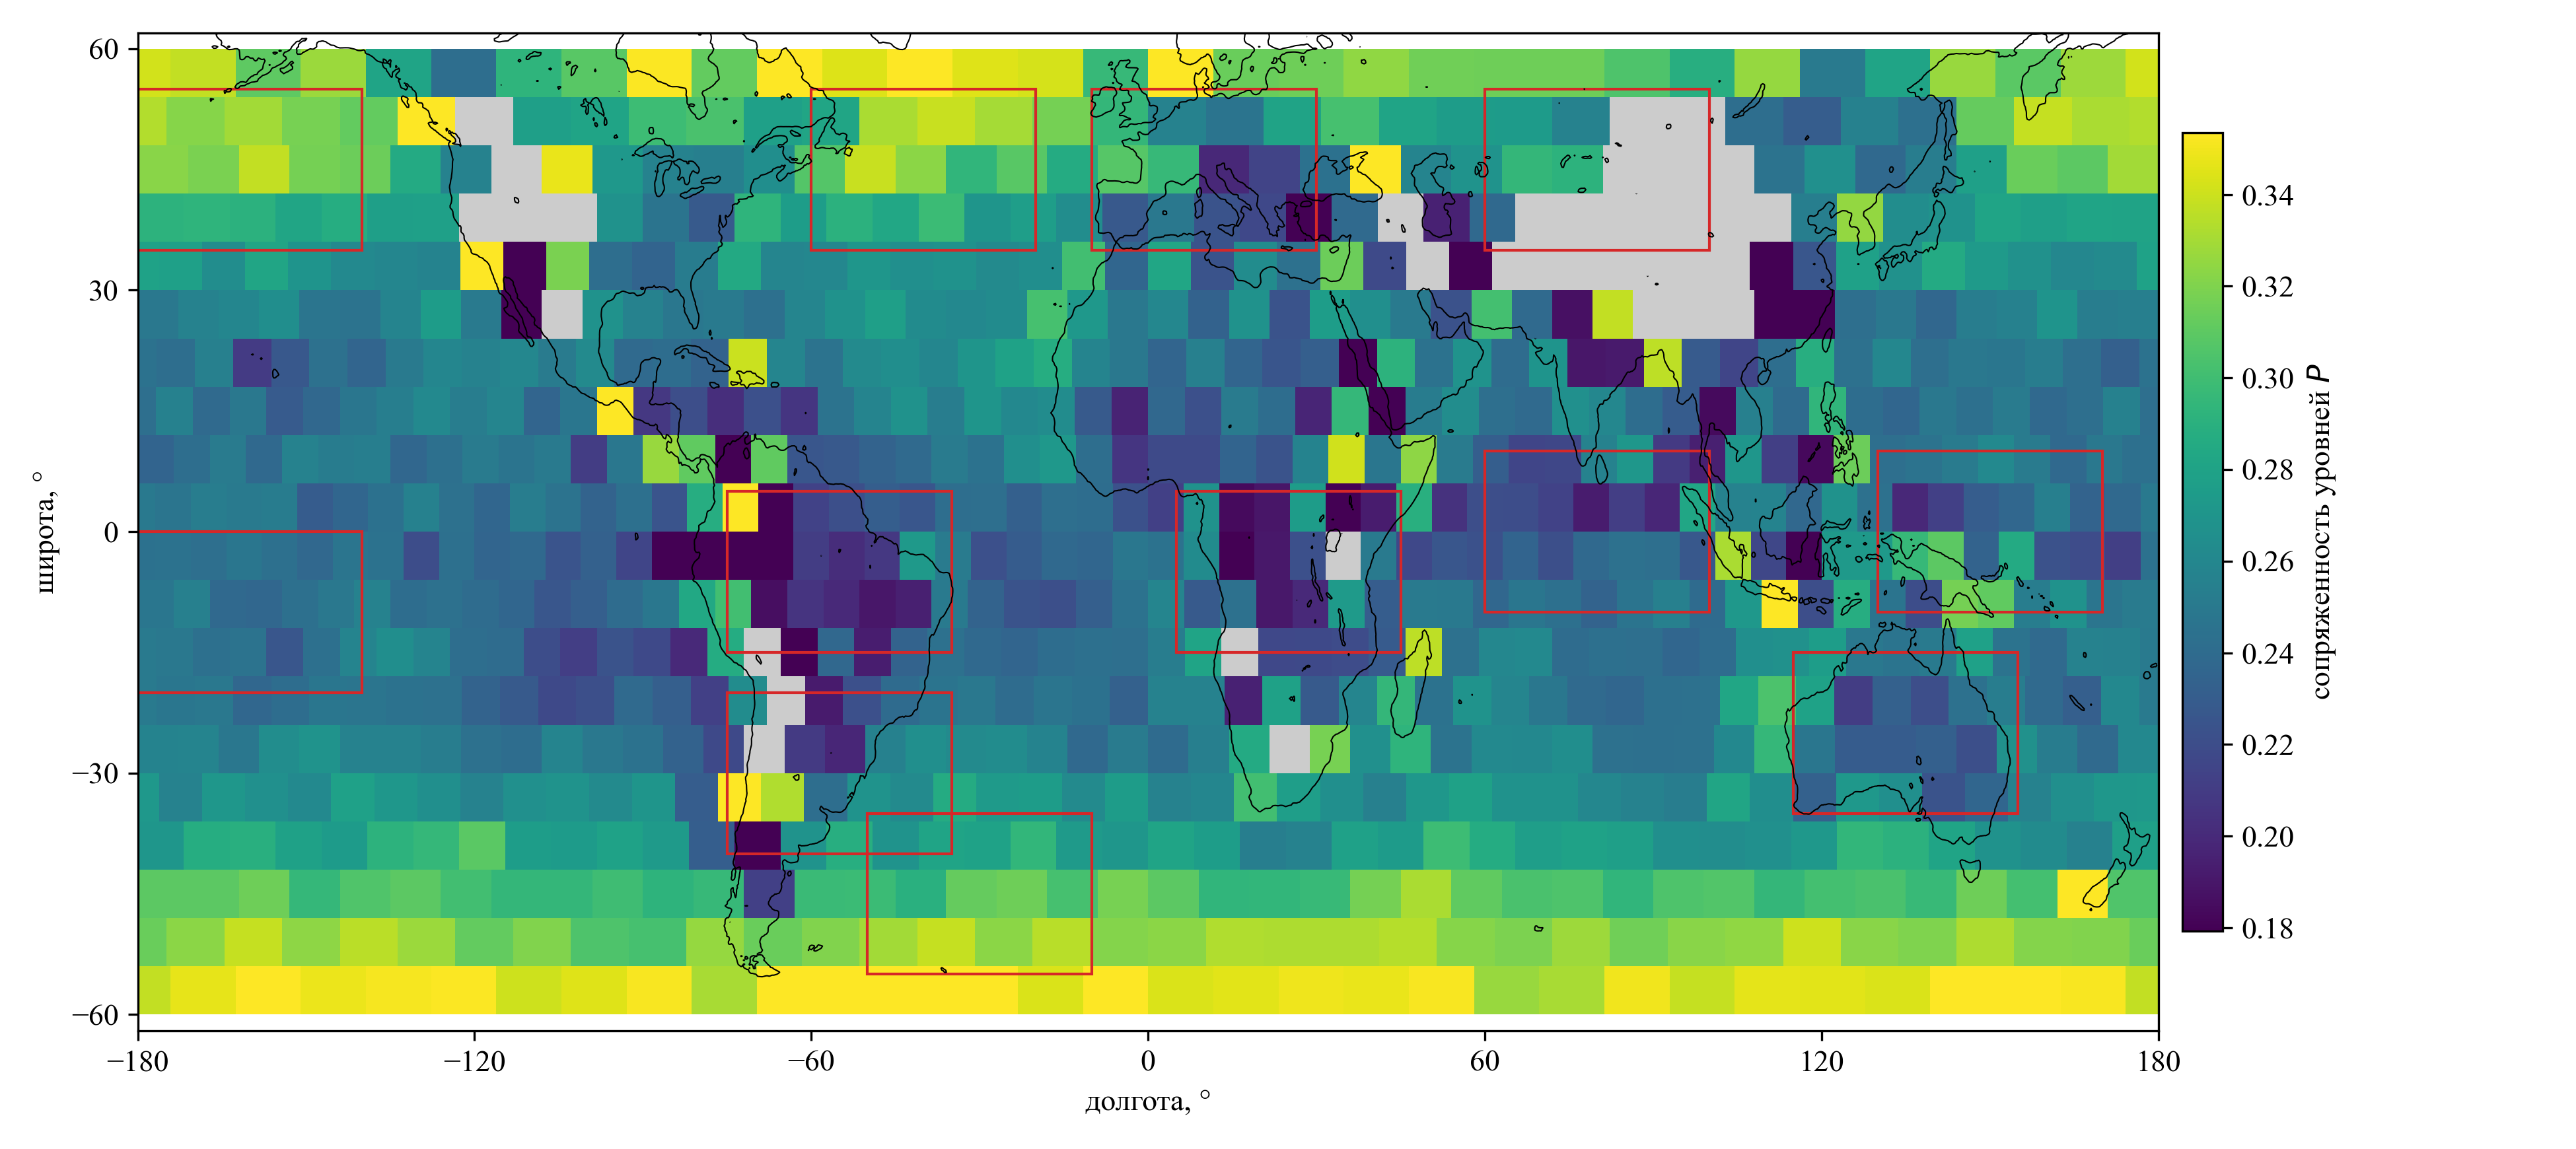
\includegraphics[width=\linewidth]{figures/ru_fig1_global_map.png}

\noindent Рис. 1. Планетарная карта сопряженности масштабных уровней $P$ (масштабы 50--400 км): среднее по сезонам январь--март и июль--сентябрь 2023 г., 936 ячеек между 60$^\circ$ ю.ш. и 60$^\circ$ с.ш. Серым показаны ячейки, исключенные из-за высоты рельефа более 1200 м; красные рамки -- двенадцать областей первой статьи.

\clearpage
\noindent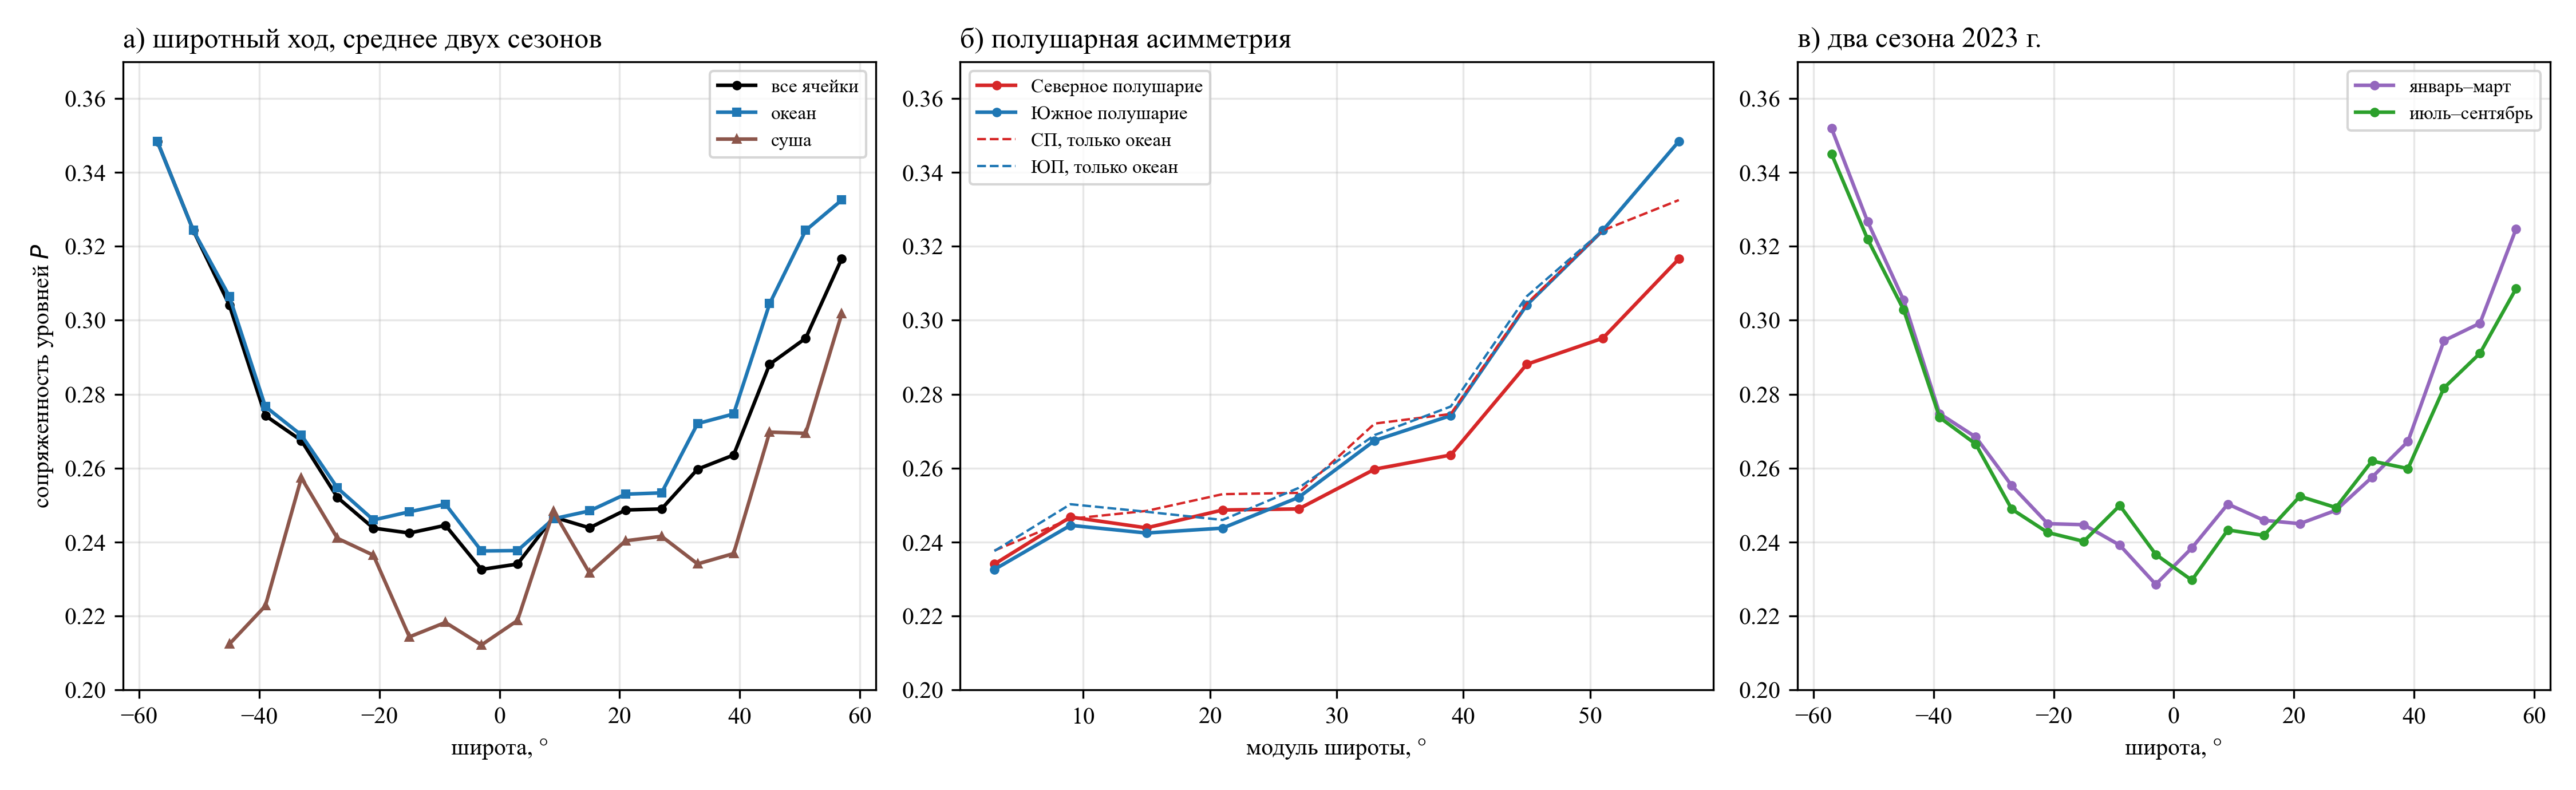
\includegraphics[width=\linewidth]{figures/fig2_zonal_profiles.png}

\noindent Рис. 2. Широтная структура карты (902 ячейки): а -- средние значения по полосам 6$^\circ$ для всех ячеек, для океана и для суши; б -- средние значения по модулю широты для Северного и Южного полушарий (сплошные линии -- все ячейки, штриховые -- только океан); в -- широтный ход в сезоны январь--март и июль--сентябрь 2023 г.

\clearpage
\noindent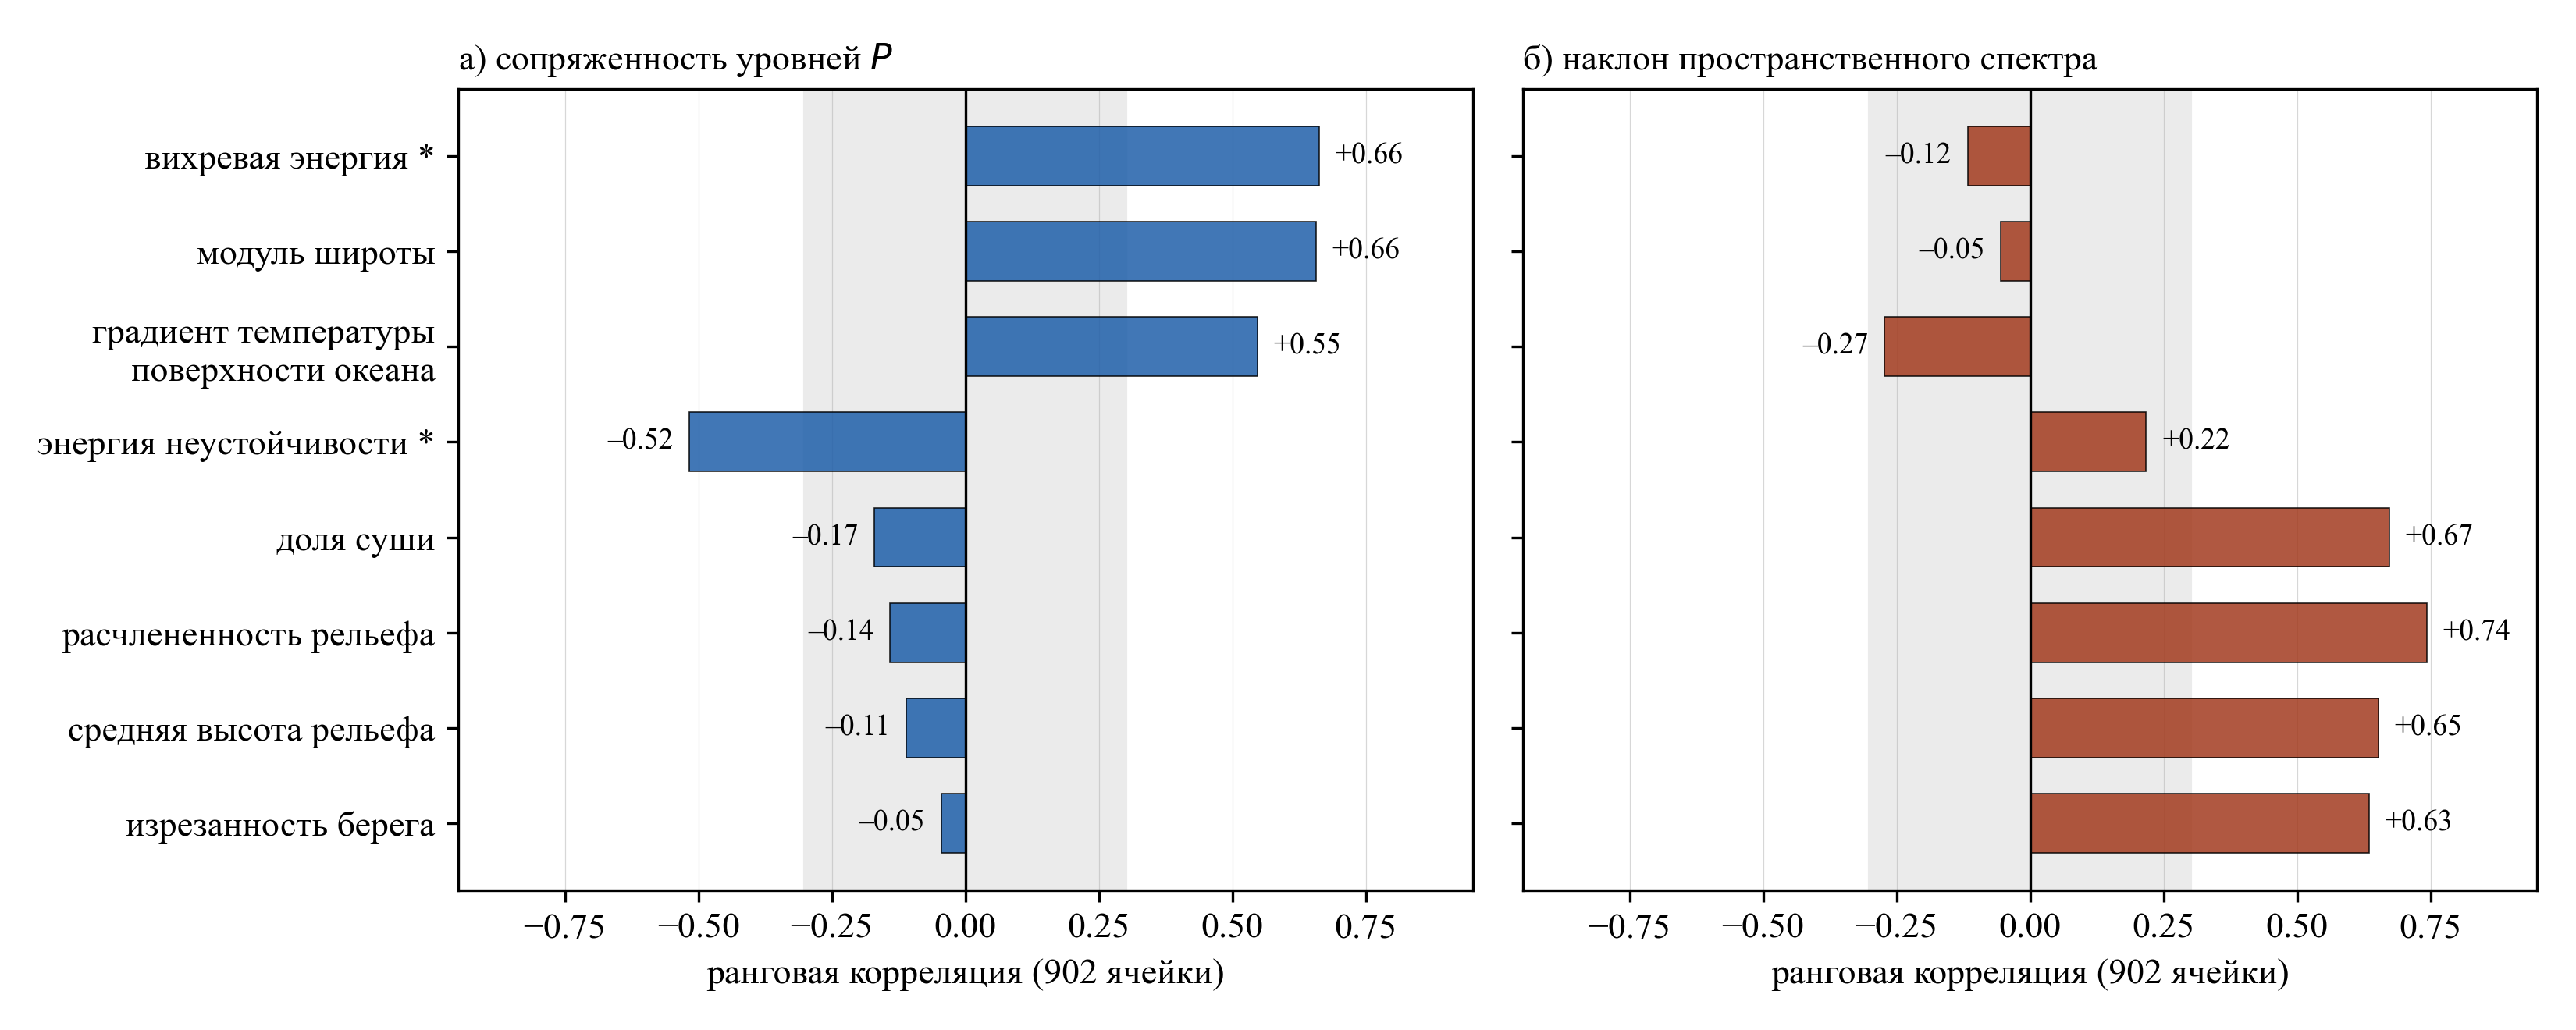
\includegraphics[width=\linewidth]{figures/ru_fig3_channels.png}

\noindent Рис. 3. Связь восьми факторов с сопряженностью уровней (а) и с наклоном пространственного спектра (б): ранговая корреляция по 902 ячейкам. Серая полоса -- значения корреляции по модулю менее 0.3. Звездочкой отмечены характеристики циркуляционного режима, остальные факторы -- стационарные свойства территории.

\clearpage
\noindent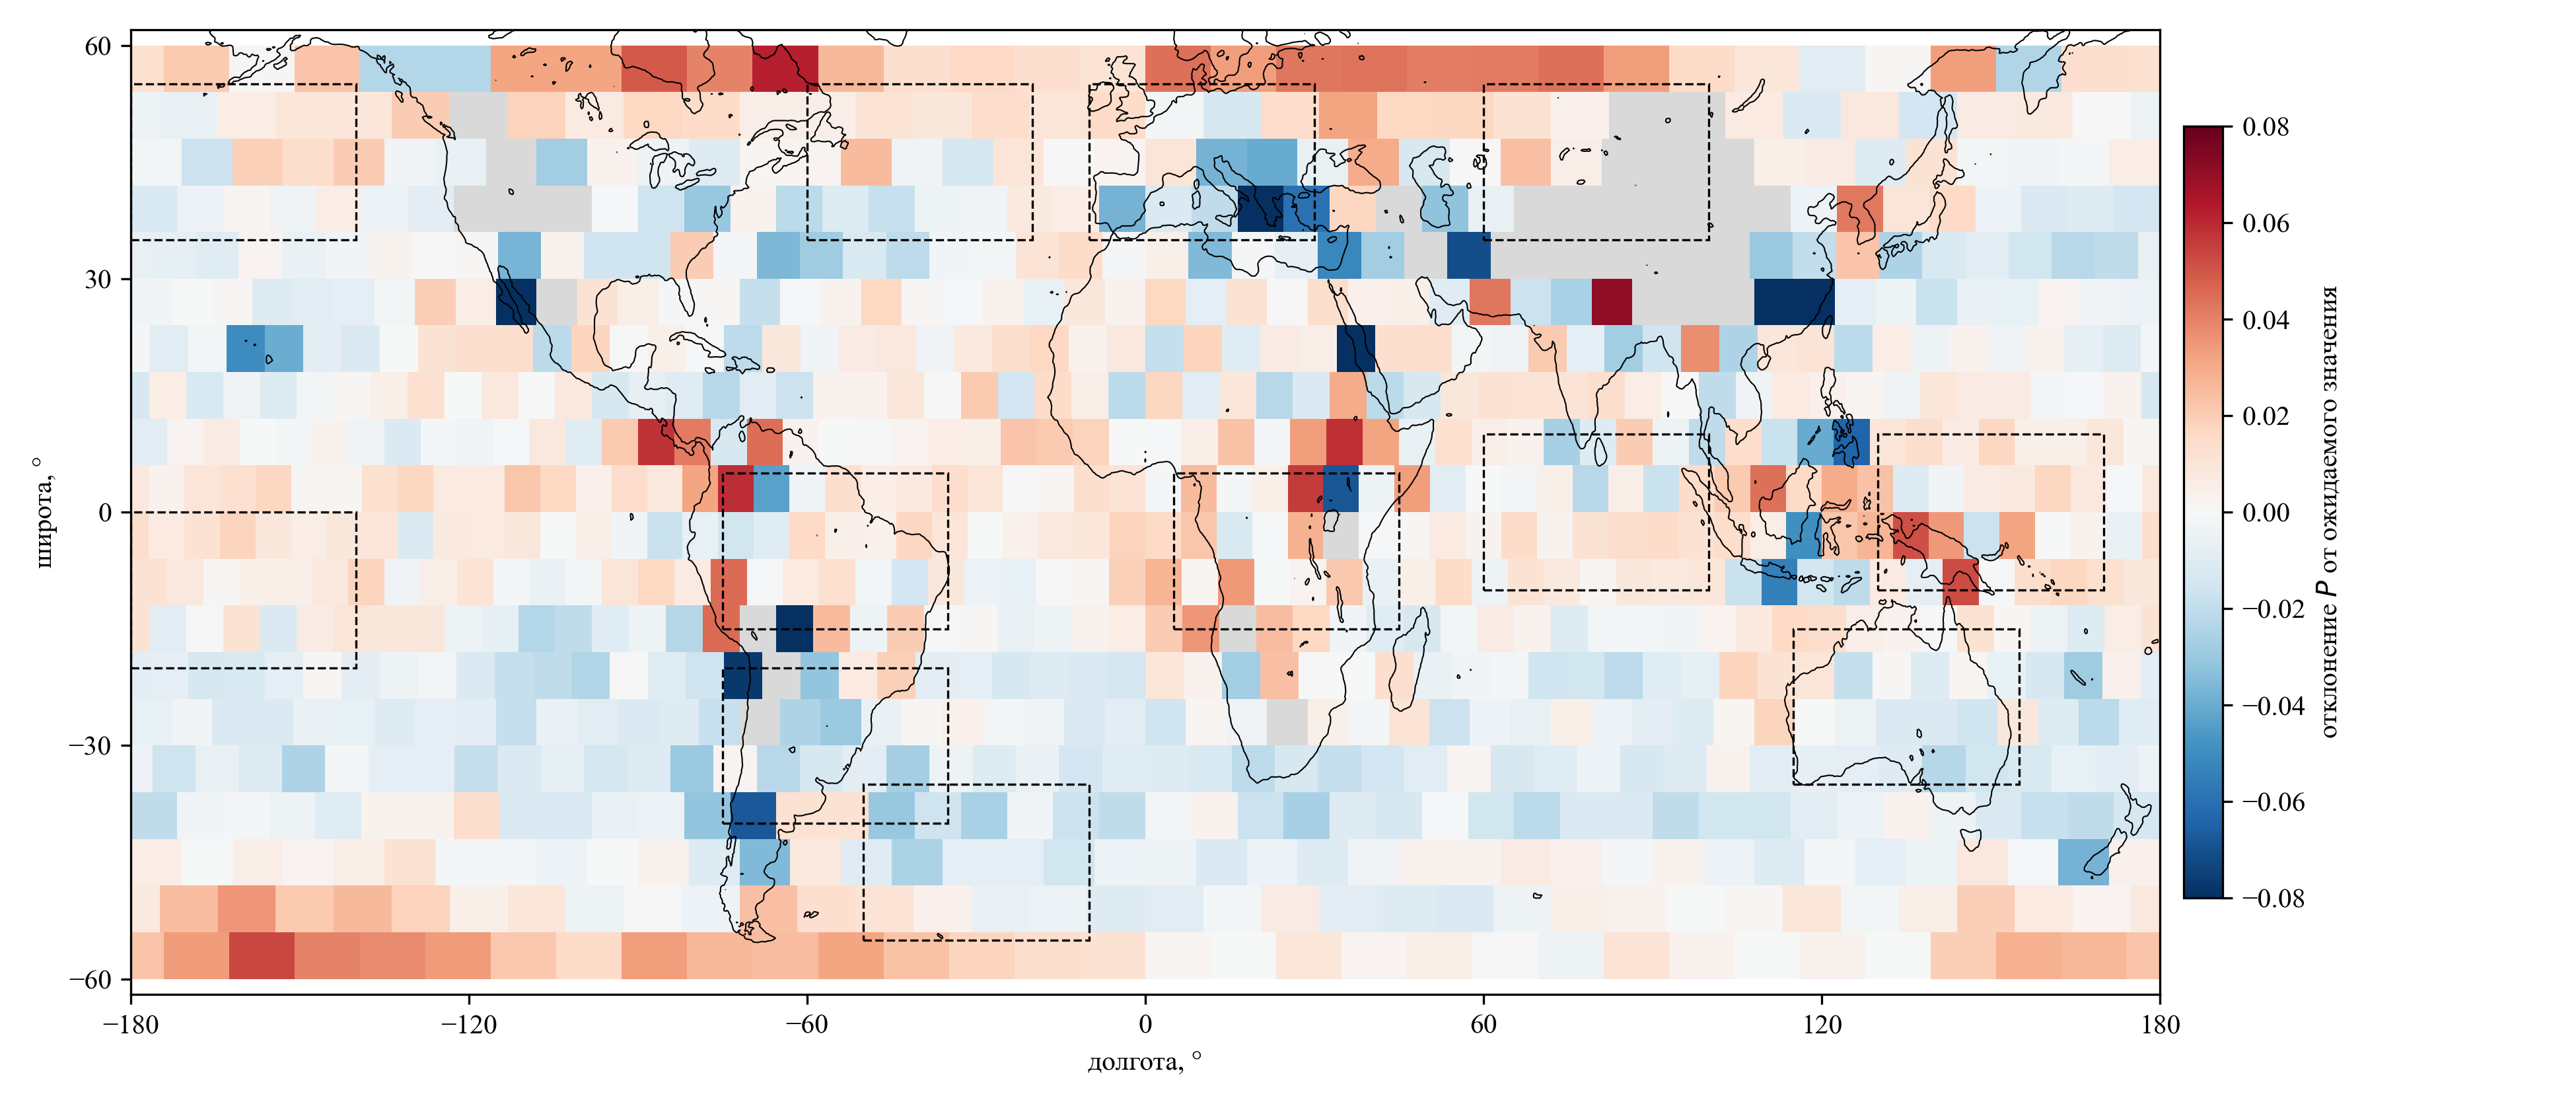
\includegraphics[width=\linewidth]{figures/fig2_residual_map.png}

\noindent Рис. 4. Необъясненная часть карты: отклонение сопряженности от значения, ожидаемого по восьми факторам и статистикам перемежаемости (среднее по двум сезонам 2023 г.). Синим показаны значения ниже ожидаемых, красным -- выше ожидаемых. Серым показаны исключенные ячейки; штриховые рамки -- двенадцать областей первой статьи.

\clearpage
\noindent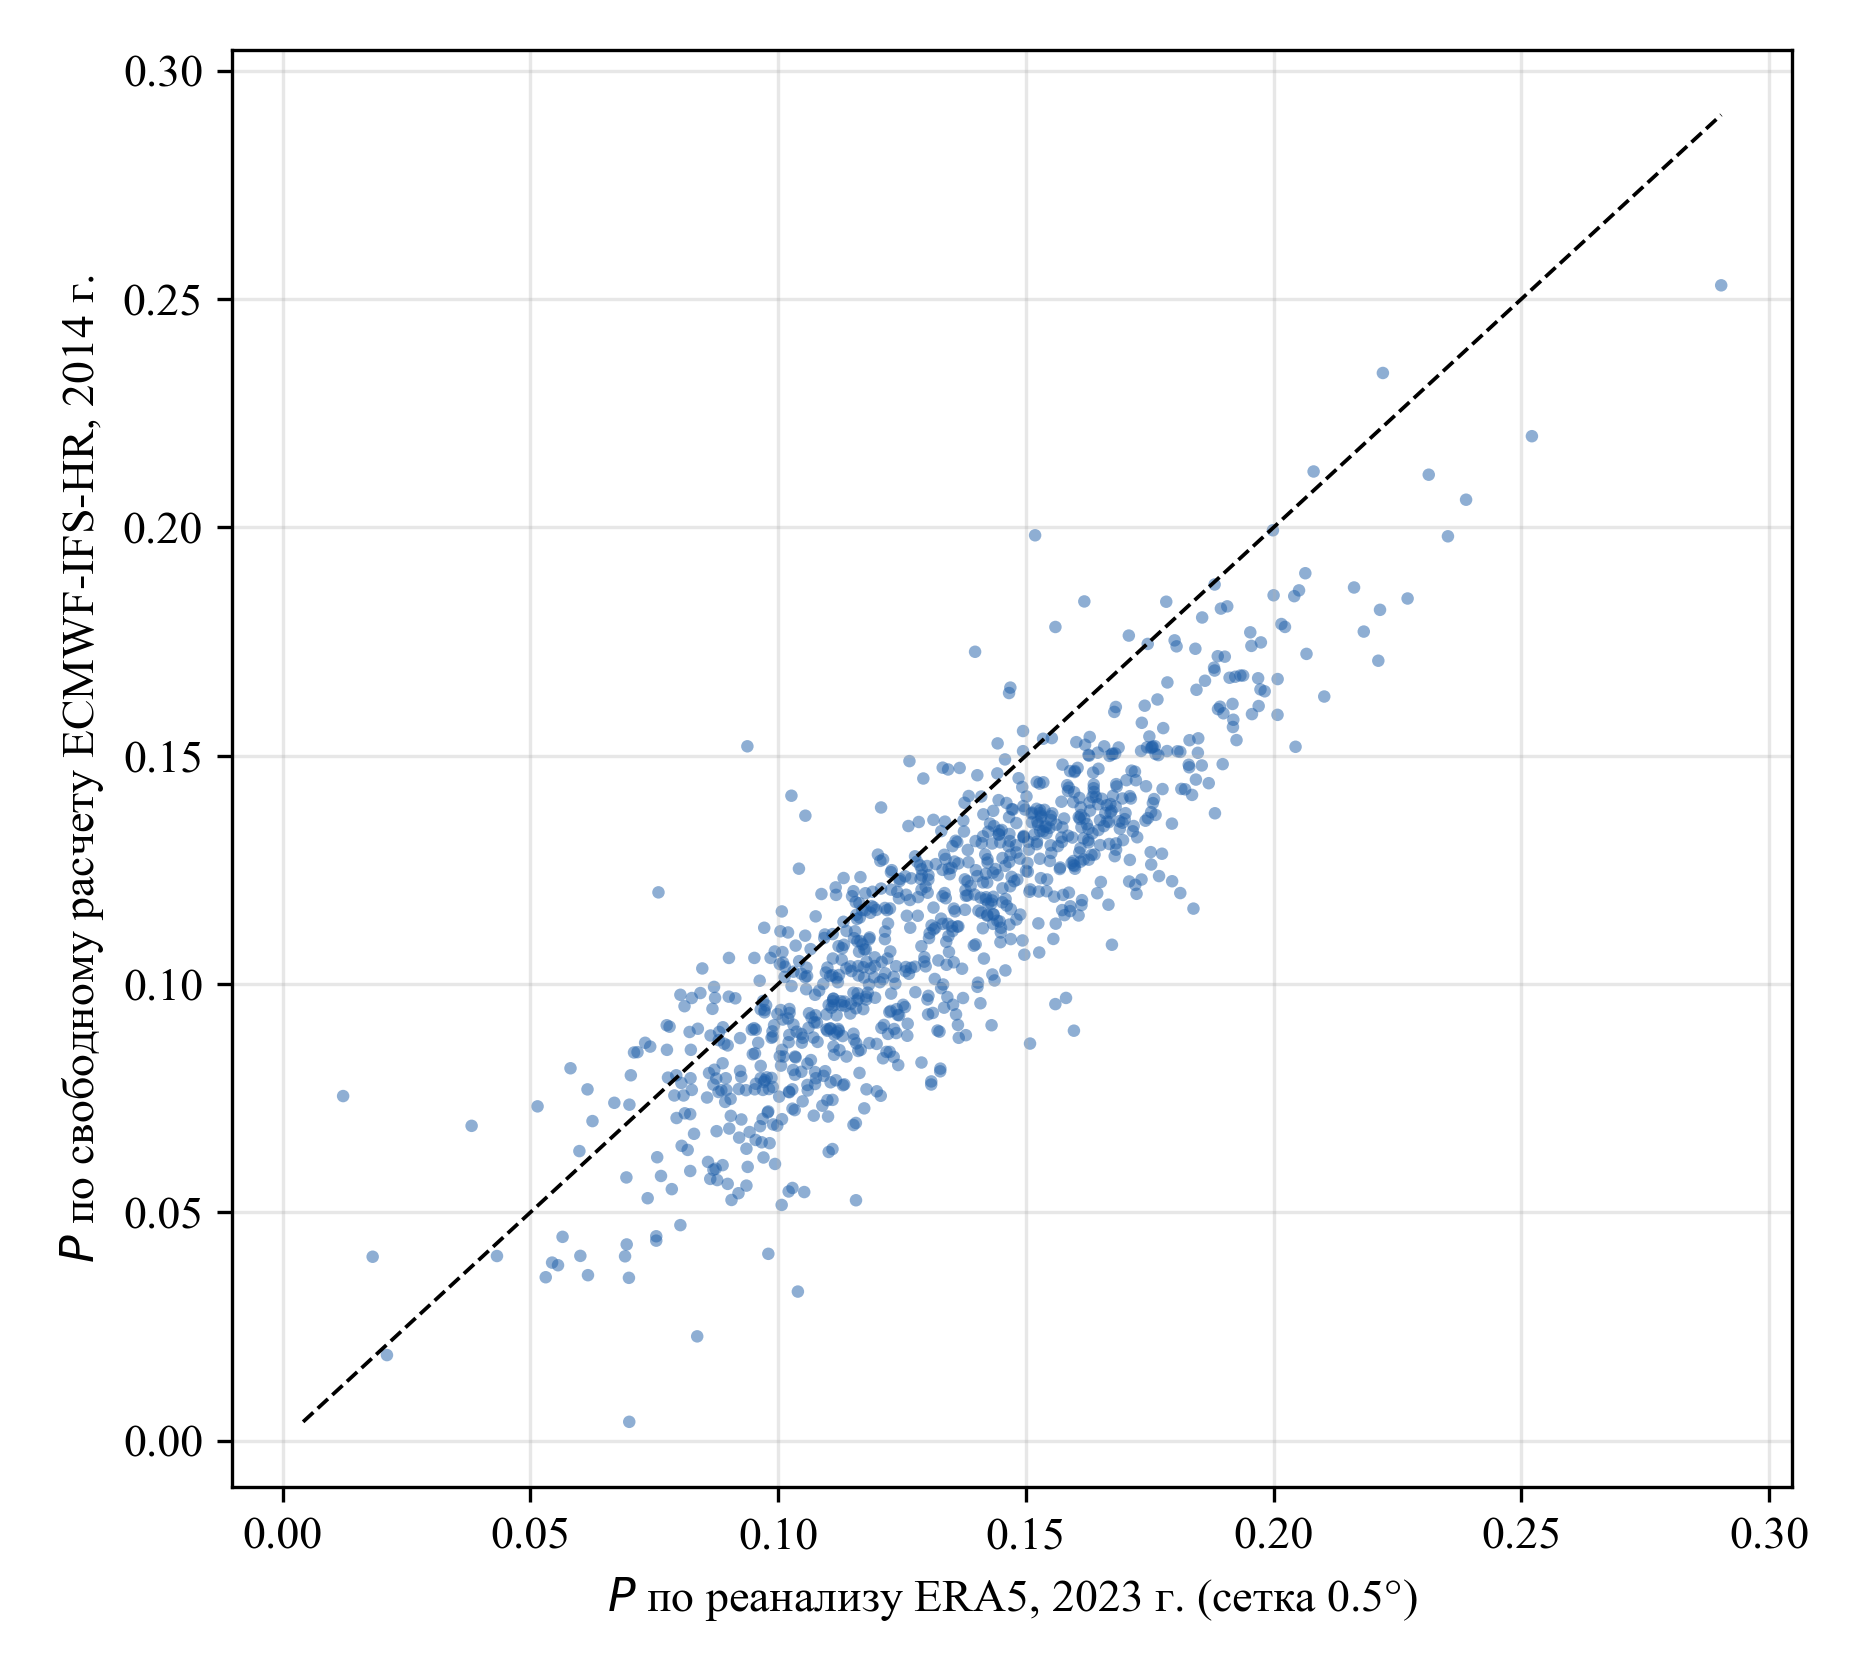
\includegraphics[width=0.7\linewidth]{figures/ru_fig5_model.png}

\noindent Рис. 5. Сопоставление карты сопряженности по модельному расчету без усвоения наблюдений (ECMWF-IFS-HR, 2014 г.) и по реанализу ERA5 (2023 г.) для 902 ячеек. Каждая точка -- одна ячейка; штриховая линия -- линия равных значений. Ранговая корреляция равна 0.87.

\clearpage
\noindent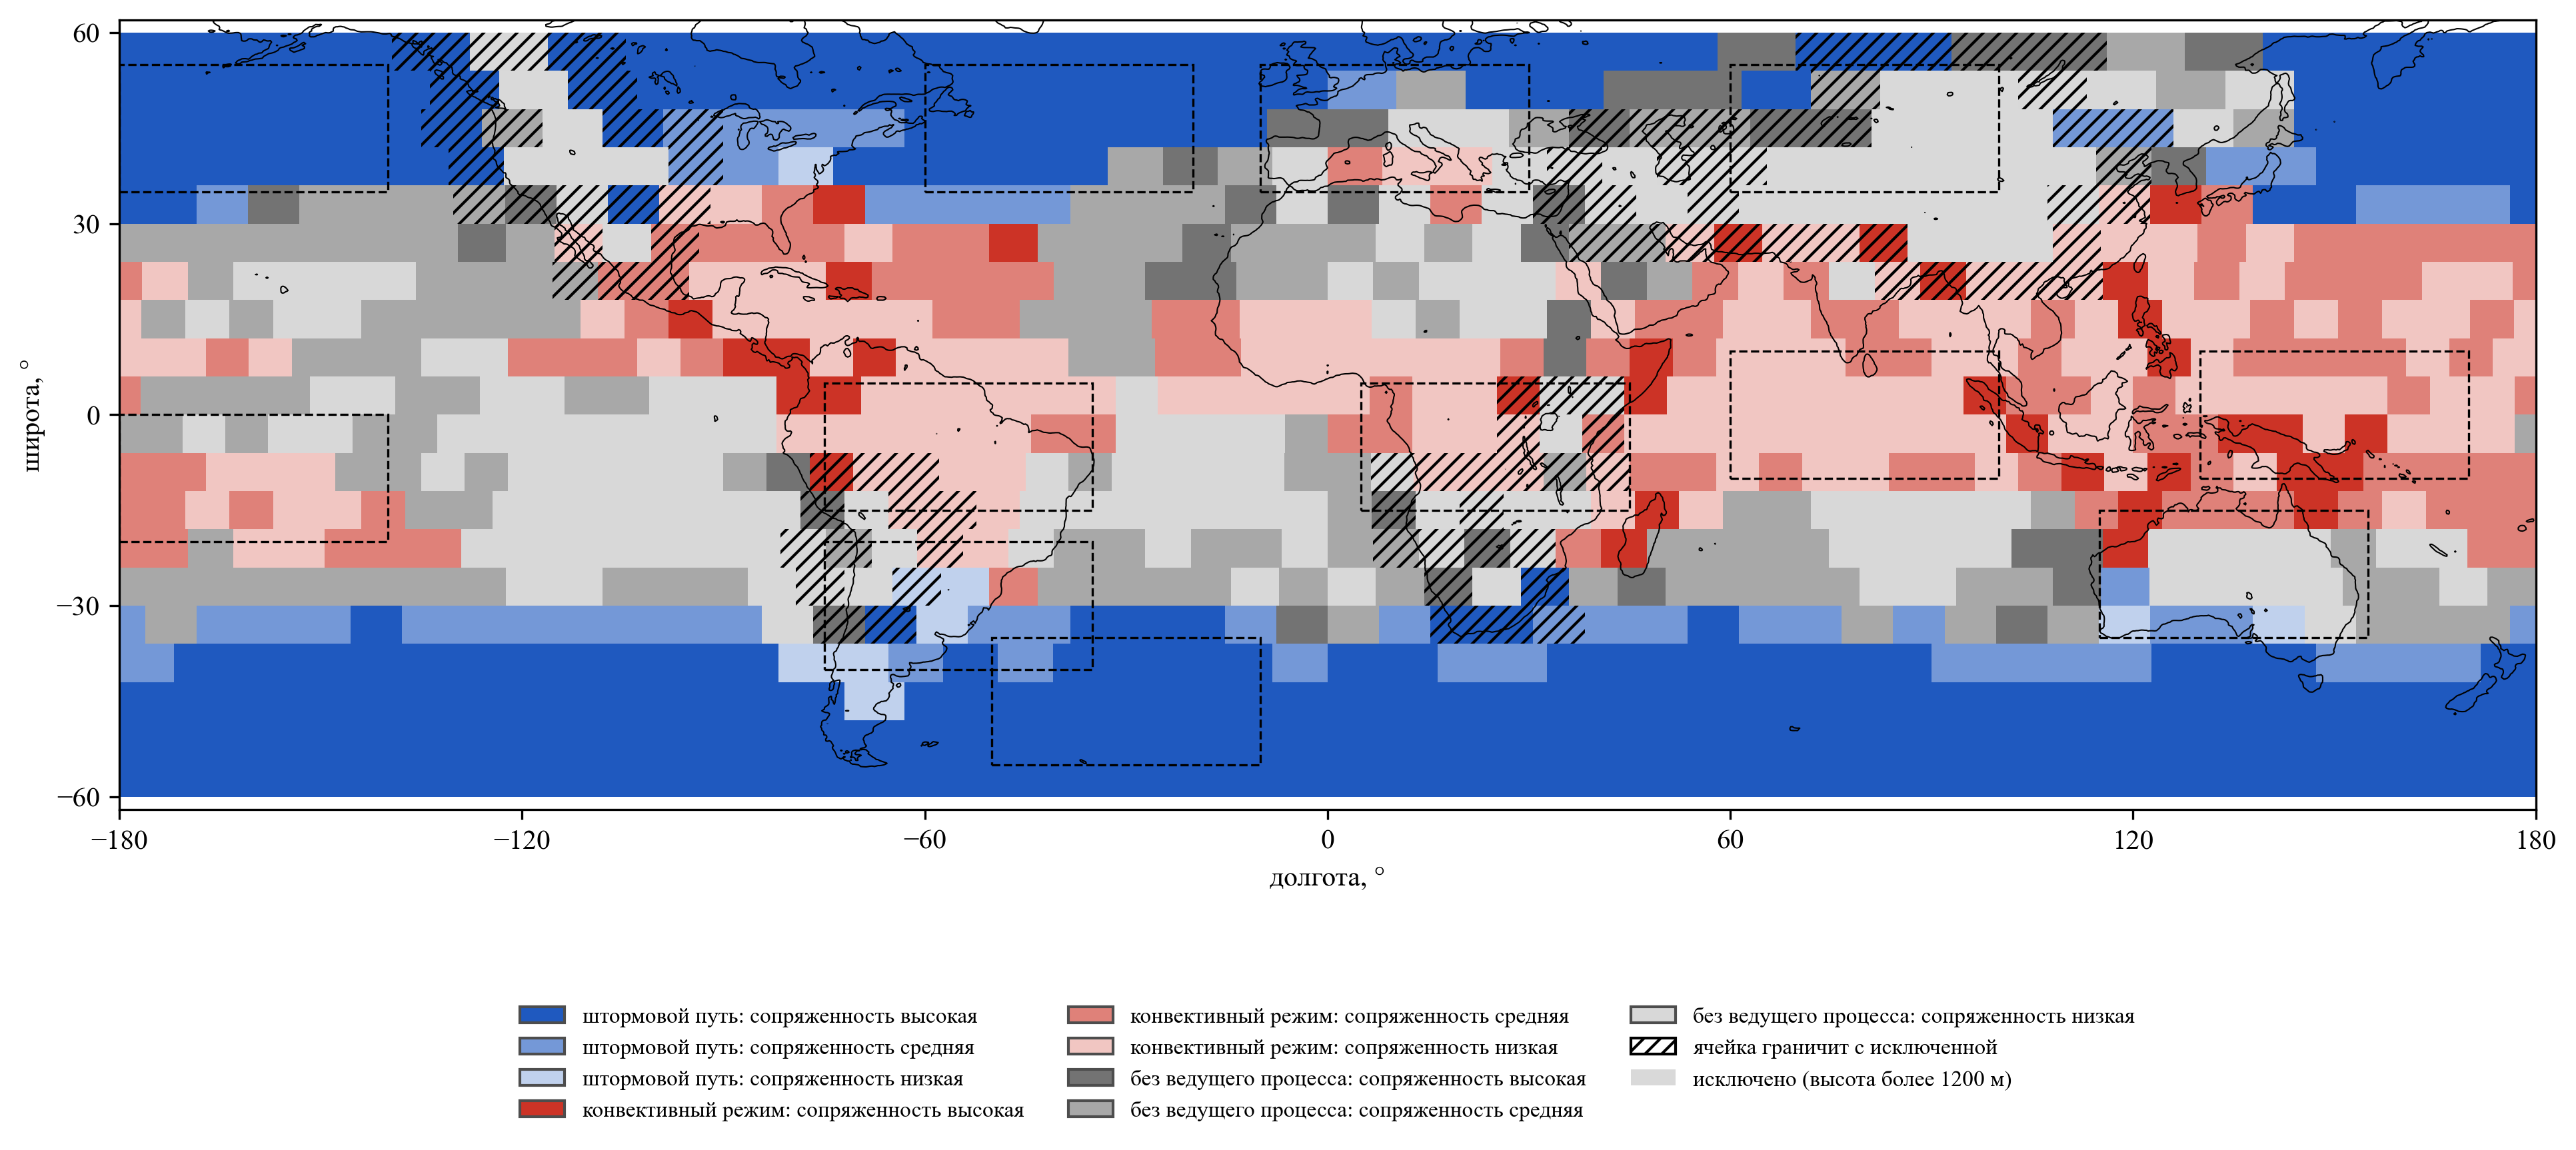
\includegraphics[width=\linewidth]{figures/fig2_regionalization.png}

\noindent Рис. 6. Схема районирования по сопряженности уровней. Цвет обозначает ведущий циркуляционный процесс: синий -- штормовой путь, красный -- конвективный режим, серый -- процесс не выражен. Насыщенность цвета обозначает уровень сопряженности: темный тон -- высокая, светлый -- низкая. Штриховкой отмечены ячейки, граничащие с исключенными; светло-серым показаны исключенные ячейки; штриховые рамки -- двенадцать областей первой статьи.

\clearpage
\begin{center}
{\large\bfseries Geography of the coupling between hierarchical levels of the atmospheric circulation: a planetary map, its controls and a regionalisation}

\medskip
{\bfseries N. S. Sotiriadi\textsuperscript{*}}

Independent researcher, Moscow, Russia

\textsuperscript{*}E-mail: n.sotiriadi@gmail.com
\end{center}

\begin{singlespace}
\noindent\textbf{Abstract.} The coupling of neighbouring scale levels of the atmospheric circulation shows how far the placement of mesoscale variability is set by the adjacent larger level. It was previously established as a stable characteristic of a territory. The aim of this paper is to build a planetary map of the coupling, to explain its geography and to propose a regionalisation scheme that can be used alongside the accepted climatic and landscape criteria. The map is built from the ERA5 relative-vorticity field at 850 hPa for 936 cells of about 667 by 700 km between 60$^\circ$S and 60$^\circ$N for two seasons of 2023. The highest values form a continuous ring over the Southern Ocean and areas over the North Pacific and North Atlantic. The lowest values sit over the deep-convective cores of Amazonia, the Congo basin and the Maritime Continent and over the subtropical monsoon lands. Coupling rises from the equator to mid-latitudes and is higher over ocean than over land in every belt. The mid-latitude difference between the hemispheres is explained by the distribution of land. In the tropics coupling decreases in the wet season. The geography of the map is governed mainly by extratropical cyclone activity, which raises coupling, and by deep convection, which lowers it. Stationary properties of the territory -- latitude, sea-surface temperature, the land--sea distribution -- recover the map almost as well. A model integration that assimilates no observations reproduces the map, so it reflects a property of the atmosphere. A typology of territories by leading circulation process and coupling level is proposed. It singles out provinces that are indistinguishable by standard regime characteristics: the continental margins of the storm tracks, coastal areas of organised convection, and upwelling coasts.

\smallskip
\noindent\textbf{Keywords:} extratropical cyclones, deep convection, monsoon, reanalysis, mesoscale variability, latitudinal zonality, land and ocean, typology of territories, provinces, model integration.

\smallskip
\noindent\textbf{Funding.} The study received no external funding. The author declares no conflict of interest.
\end{singlespace}

\end{document}
